\documentclass[11pt,letterpaper]{article}

\usepackage[utf8]{inputenc}
\usepackage[T1]{fontenc}
\usepackage{lmodern}
\usepackage[margin=1in]{geometry}
\usepackage{amsmath}
\usepackage{graphicx}
\usepackage{booktabs}
\usepackage{siunitx}
\usepackage{xcolor}
\usepackage[numbers,sort&compress]{natbib}
\usepackage[colorlinks=true,linkcolor=blue!50!black,citecolor=blue!50!black,urlcolor=blue!50!black]{hyperref}

\sisetup{group-separator={,},group-minimum-digits=4}
\graphicspath{{../benchmark/results/}}

% Placeholder for content that awaits final results
\newcommand{\todo}[1]{\textcolor{red}{[TODO: #1]}}

\title{Performance of GPU-Accelerated VASP 6.5.1 on a Dual NVIDIA H100 Node:\\
Materials Project PBE and r\textsuperscript{2}SCAN Workflows, and Finite-Displacement Phonons}
\author{Gilles Frapper \\ Professor, Theoretical Chemistry \\ IC2MP UMR 7285 CNRS, Universit\'e de Poitiers \\ \href{mailto:gilles.frapper@univ-poitiers.fr}{gilles.frapper@univ-poitiers.fr}}
\date{Draft, September 27, 2026}

\begin{document}
\maketitle

\begin{abstract}
\todo{Write once all results are final (2-GPU series and phonons).}
We benchmark the GPU (OpenACC) build of VASP 6.5.1 on a shared node with two NVIDIA H100 NVL
GPUs. Single-point and full cell relaxation calculations are run on supercell series of Si, Al,
and MgO from 1 to 64 atoms, using the Materials Project PBE and r\textsuperscript{2}SCAN input
sets. We report wall time, time per self-consistent step, GPU memory, the cost of
r\textsuperscript{2}SCAN relative to PBE, the speedup from one to two GPUs with two
parallelization strategies, run-to-run reproducibility, and agreement with published Materials
Project energies. Finite-displacement phonon calculations complete the study.
\end{abstract}

% ---------------------------------------------------------------------------
\section{Introduction}
\label{sec:intro}

\todo{Context: GPU ports of plane-wave DFT codes; high-throughput workflows such as Materials
Project~\cite{Jain2013}; practical questions for a small shared GPU node.}

This study addresses the following questions:
\begin{enumerate}
  \item How does computing time scale with the number of atoms, from 1 to 64?
  \item How much more does r\textsuperscript{2}SCAN cost than PBE, per self-consistent (SCF)
        step and in total?
  \item How much does a full relaxation cost compared with a single point?
  \item What is gained by going from one to two GPUs, and is it better to distribute
        $k$-points (\texttt{KPAR}=2) or bands and plane waves (\texttt{KPAR}=1)?
  \item How much GPU memory is needed as a function of system size?
  \item Are timings reproducible from one job to the next?
  \item Are the computed energies consistent with those published by Materials Project?
  \item What is the time-to-solution of a complete finite-displacement phonon calculation on one
        and two GPUs?
\end{enumerate}

% ---------------------------------------------------------------------------
\section{Hardware and Software}
\label{sec:hardware}

\begin{table}[htbp]
\centering
\caption{Test system.}
\label{tab:hardware}
\small
\begin{tabular}{@{}ll@{}}
\toprule
Component & Specification \\
\midrule
GPUs & 2 $\times$ NVIDIA H100 NVL, \SI{94}{GB} each (driver 595.84) \\
CPU & AMD EPYC 7662, 32 cores assigned to the virtual machine \\
Host memory & \SI{62}{GB} \\
Per GPU (Slurm) & 16 cores, $\sim$\SI{28}{GB} host memory, no time limit \\
DFT code & VASP 6.5.1, OpenACC GPU build \\
Toolchain & NVIDIA HPC SDK 26.3, HPC-X (CUDA-aware Open MPI), Intel oneMKL \\
Execution & one MPI rank per GPU, \texttt{OMP\_NUM\_THREADS}=1 \\
Workflow tools & pymatgen 2026.9.23~\cite{Ong2013}, phonopy 4.6.0~\cite{Togo2023,Togo2015} \\
\bottomrule
\end{tabular}
\end{table}

The node is shared with other users through Slurm. To leave the second GPU available, study jobs
were submitted as job arrays running one calculation at a time. One-GPU and two-GPU series were
never submitted concurrently. For each
calculation, the jobs running on the node at start time were recorded, since they may affect
timings (Section~\ref{sec:metrics}).

% ---------------------------------------------------------------------------
\section{Methods}
\label{sec:methods}

\subsection{Structures}
\label{sec:structures}

All structures were retrieved from Materials Project~\cite{Jain2013} (Table~\ref{tab:structures}).
To isolate the effect of system size at constant chemistry, each material is studied as a series
of supercells of increasing size, 14 structures in total. The MP structures are already relaxed
with PBE.

\begin{table}[htbp]
\centering
\caption{Scaling series.}
\label{tab:structures}
\begin{tabular}{@{}llll@{}}
\toprule
Material & MP ID & Type & Sizes (atoms) \\
\midrule
Si, diamond & mp-149 & semiconductor (PBE gap \SI{0.61}{eV}) & 2 (primitive), 8, 16, 32, 64 \\
Al, fcc & mp-134 & metal & 1 (primitive), 4, 32, 64 \\
MgO, rock salt & mp-1265 & insulator (PBE gap \SI{4.43}{eV}) & 2 (primitive), 8, 16, 32, 64 \\
\bottomrule
\end{tabular}
\end{table}

\subsection{Electronic-structure settings}
\label{sec:settings}

All calculations use the projector augmented-wave (PAW) method~\cite{Blochl1994,Kresse1999} as
implemented in VASP~\cite{Kresse1996}. Inputs were generated with the Materials Project input
sets implemented in pymatgen~\cite{Ong2013}, without changing any physical parameter
(Table~\ref{tab:sets}). The PBE sets~\cite{Perdew1996} apply the MP Hubbard $U$
values~\cite{Dudarev1998} to oxides and fluorides of Co, Cr, Fe, Mn, Mo, Ni, and V (none of the
present materials is affected). The r\textsuperscript{2}SCAN sets~\cite{Furness2020} follow the
MP meta-GGA workflow~\cite{Kingsbury2022}, in which the $k$-point spacing is chosen from the MP
band gap. All calculations are spin-polarized (\texttt{ISPIN}=2), with \texttt{PREC}=Accurate
and \texttt{LASPH}=.TRUE.

\begin{table}[htbp]
\centering
\caption{Calculation series and main parameters. Brillouin-zone sampling is expressed per
reciprocal-lattice volume (PBE) or as \texttt{KSPACING} (r\textsuperscript{2}SCAN).}
\label{tab:sets}
\small
\begin{tabular}{@{}llp{9.2cm}@{}}
\toprule
Series & pymatgen set & Main parameters \\
\midrule
\texttt{pbe\_sp} & \texttt{MPStaticSet} & PBE; \texttt{ENCUT}=\SI{520}{eV}; 100 $k$-points per
\si{\angstrom^{-3}}; \texttt{EDIFF}=\SI{5e-5}{eV} per atom; \texttt{ALGO}=Fast;
\texttt{LREAL}=.FALSE. \\
\texttt{pbe\_relax} & \texttt{MPRelaxSet} & as above, with \texttt{ISIF}=3, \texttt{IBRION}=2;
64 $k$-points per \si{\angstrom^{-3}}; \texttt{LREAL}=Auto \\
\texttt{r2scan\_sp} & \texttt{MPScanStaticSet} & \texttt{METAGGA}=R2SCAN;
\texttt{ENCUT}=\SI{680}{eV}; \texttt{KSPACING} from 0.22 to \SI{0.44}{\angstrom^{-1}}
depending on the MP gap; \texttt{EDIFF}=\SI{1e-5}{eV} \\
\texttt{r2scan\_relax} & \texttt{MPScanRelaxSet} & as above, with \texttt{ISIF}=3,
\texttt{ALGO}=All, \texttt{EDIFFG}=\SI{-0.02}{eV/\angstrom} \\
\bottomrule
\end{tabular}
\end{table}

The following deviations from the MP methodology apply identically to every calculation:
\begin{itemize}
  \item \textbf{Pseudopotentials.} The PBE\_54 PAW set installed on the machine is used for
        both functionals. MP uses an older PBE set for its GGA calculations, which is identical
        for almost all elements; W\_pv, absent from PBE\_54, would be replaced by W\_sv.
  \item \textbf{Output.} Writing of \texttt{WAVECAR}, \texttt{CHGCAR}, \texttt{AECCAR},
        \texttt{LOCPOT}, and \texttt{ELFCAR} is disabled, so that the benchmark measures
        computation rather than I/O.
  \item \textbf{Parallelization tags.} \texttt{NCORE} is removed, since the GPU build forces it
        to 1; \texttt{KPAR} is set by the parallelization variant
        (Section~\ref{sec:variants}).
  \item \textbf{Small $k$-point meshes.} When a mesh has fewer than 4 irreducible $k$-points,
        the tetrahedron method (\texttt{ISMEAR}=$-5$) is replaced by Gaussian smearing
        (\texttt{ISMEAR}=0, \texttt{SIGMA}=\SI{0.05}{eV}), which is also the correction
        applied by custodian in MP workflows.
\end{itemize}

In the supercells, the $k$-point density per atom is kept constant, as in the MP methodology,
so the number of $k$-points decreases as the cell grows. Relaxations start from the MP
structures, which are already relaxed with PBE: PBE relaxations therefore converge in a few
ionic steps, and r\textsuperscript{2}SCAN relaxations need a few more.

\subsection{Parallelization variants}
\label{sec:variants}

Three variants are compared (Table~\ref{tab:variants}), with identical physical inputs. With two
GPUs, \texttt{KPAR}=1 distributes bands and plane-wave coefficients across both devices, while
\texttt{KPAR}=2 assigns one group of $k$-points to each GPU. The \texttt{g2k2} variant is
skipped when a structure has fewer than two irreducible $k$-points.

\begin{table}[htbp]
\centering
\caption{Parallelization variants.}
\label{tab:variants}
\begin{tabular}{@{}lccc@{}}
\toprule
Variant & GPUs & MPI ranks & \texttt{KPAR} \\
\midrule
\texttt{g1} & 1 & 1 & 1 \\
\texttt{g2k1} & 2 & 2 & 1 \\
\texttt{g2k2} & 2 & 2 & 2 \\
\bottomrule
\end{tabular}
\end{table}

\subsection{Measurement protocol}
\label{sec:metrics}

Each calculation runs as one Slurm job-array task launched with
\texttt{mpirun -np $N_\text{GPU}$ --bind-to none vasp\_std}. The following quantities are
recorded:
\begin{itemize}
  \item \textbf{Problem size:} number of atoms, \texttt{NKPTS}, \texttt{NBANDS}, \texttt{NPLWV},
        \texttt{NELECT}, \texttt{ISPIN}.
  \item \textbf{Time:} total time (``Elapsed time'' in \texttt{OUTCAR}, and job wall time);
        median time per SCF step (\texttt{LOOP} lines); mean time per ionic step
        (\texttt{LOOP+} lines); numbers of SCF and ionic steps.
  \item \textbf{Memory and utilization:} peak GPU memory and mean GPU utilization, sampled
        every \SI{2}{s} with \texttt{nvidia-smi}; peak host memory.
  \item \textbf{Energy:} energy per atom and its difference from the uncorrected MP energy of
        the same functional, in meV/atom.
  \item \textbf{Context:} other jobs running on the node at start time.
\end{itemize}

The speedup of a two-GPU variant is the ratio of the one-GPU total time to the two-GPU total
time. Reproducibility was assessed by repeating six single-point calculations (Si 8 atoms, Al 32
atoms, and MgO 32 atoms, with PBE and r\textsuperscript{2}SCAN) three times each on one GPU.

The study was carried out in phases, each submitted separately from the smallest to the largest
system (Table~\ref{tab:phases}).

\begin{table}[htbp]
\centering
\caption{Study phases.}
\label{tab:phases}
\begin{tabular}{@{}clcc@{}}
\toprule
Phase & Content & GPUs & Calculations \\
\midrule
0 & Workflow validation on 1--2 atoms & 1 & 5 \\
1 & Reproducibility, 3 repeats & 1 & 18 \\
2 & Single points, PBE and r\textsuperscript{2}SCAN & 1 & 28 \\
3 & Relaxations, PBE and r\textsuperscript{2}SCAN & 1 & 28 \\
4 & All four series, \texttt{g2k1} and \texttt{g2k2} & 2 & 112 \\
5 & Finite-displacement phonons, \texttt{g1} and \texttt{g2k1} & 1, 2 & 6 workflows \\
\bottomrule
\end{tabular}
\end{table}

\subsection{Finite-displacement phonons}
\label{sec:phonon-methods}

\sloppy
Harmonic phonons of the primitive cells of Si, Al, and MgO are computed with the
finite-displacement method using phonopy~\cite{Togo2023,Togo2015}. Each material is run as one
automated workflow per Slurm task, with identical inputs on one GPU (\texttt{g1}) and two GPUs
(\texttt{g2k1}, \texttt{KPAR}=1), so that only the hardware changes.

\paragraph{Settings.} \sloppy PBE with PBE\_54 PAW potentials, \texttt{ENCUT}=\SI{520}{eV},
\texttt{PREC}=Accurate, \texttt{EDIFF}=\SI{1e-8}{eV}, \texttt{ADDGRID}=.TRUE.,
\texttt{LREAL}=.FALSE., \texttt{LASPH}=.TRUE., \texttt{ALGO}=Normal, non-spin-polarized.
Gaussian smearing with $\sigma=\SI{0.01}{eV}$ is used for Si and MgO, and first-order
Methfessel--Paxton smearing with $\sigma=\SI{0.2}{eV}$ for Al. $\Gamma$-centered $k$-meshes
are built with $N_i = \max(1, \operatorname{round}(L\,|\mathbf{b}_i|))$, where $\mathbf{b}_i$ are
the reciprocal lattice vectors (without the $2\pi$ factor) and $L = \SI{50}{\angstrom}$ for
insulators and \SI{80}{\angstrom} for the metal.

\paragraph{Workflow.}
\begin{enumerate}
  \item \textbf{Tight relaxation} of the primitive cell (\texttt{ISIF}=3,
        \texttt{EDIFFG}=\SI{-1e-3}{eV/\angstrom}). The relaxation is restarted from the
        previous \texttt{CONTCAR}, which resets the plane-wave basis, until a pass completes in
        at most two ionic steps (at most four passes).
  \item \textbf{Born effective charges and $\varepsilon_\infty$} for polar materials (MgO) from
        density-functional perturbation theory (\texttt{LEPSILON}), with a finite-field
        fallback (\texttt{LCALCEPS}). They are used for the non-analytical term correction.
  \item \textbf{Force calculations} for the symmetry-irreducible displacements
        (\SI{0.01}{\angstrom}) in two diagonal supercell sizes, to check convergence
        (Table~\ref{tab:phonon-cells}).
  \item \textbf{Post-processing:} symmetrized force constants, band structure along the
        seekpath path~\cite{Hinuma2017}, density of states on a $30^3$ $q$-mesh, and
        thermodynamic properties from 0 to \SI{1000}{K}.
\end{enumerate}

\begin{table}[htbp]
\centering
\caption{Phonon supercells.}
\label{tab:phonon-cells}
\small
\begin{tabular}{@{}lcccc@{}}
\toprule
Material & Relax.\ $k$-mesh & Supercells (atoms) & Displacements & Supercell $k$-meshes \\
\midrule
Si & $16^3$ & $3^3$ (54), $4^3$ (128) & 1 per cell & $5^3$, $4^3$ \\
Al & $34^3$ & $4^3$ (64), $5^3$ (125) & 1 per cell & $9^3$, $7^3$ \\
MgO & $21^3$ & $3^3$ (54), $4^3$ (128) & 2 per cell & $7^3$, $5^3$ \\
\bottomrule
\end{tabular}
\end{table}

\paragraph{Metrics.} VASP wall time of every step and GPU-hours; time-to-solution from
submission to result, queue time included; quality checks: acoustic frequencies at $\Gamma$,
lowest frequency on the $q$-mesh (imaginary modes), and residual force drift.

% ---------------------------------------------------------------------------
\section{Results}
\label{sec:results}

\subsection{Scaling with system size on one GPU}
\label{sec:res-scaling}
\todo{Table of the 56 one-GPU calculations; Fig.~t\_total\_vs\_natoms and t\_scf\_vs\_natoms;
scaling exponents.}

% \begin{figure}[htbp]
%   \centering
%   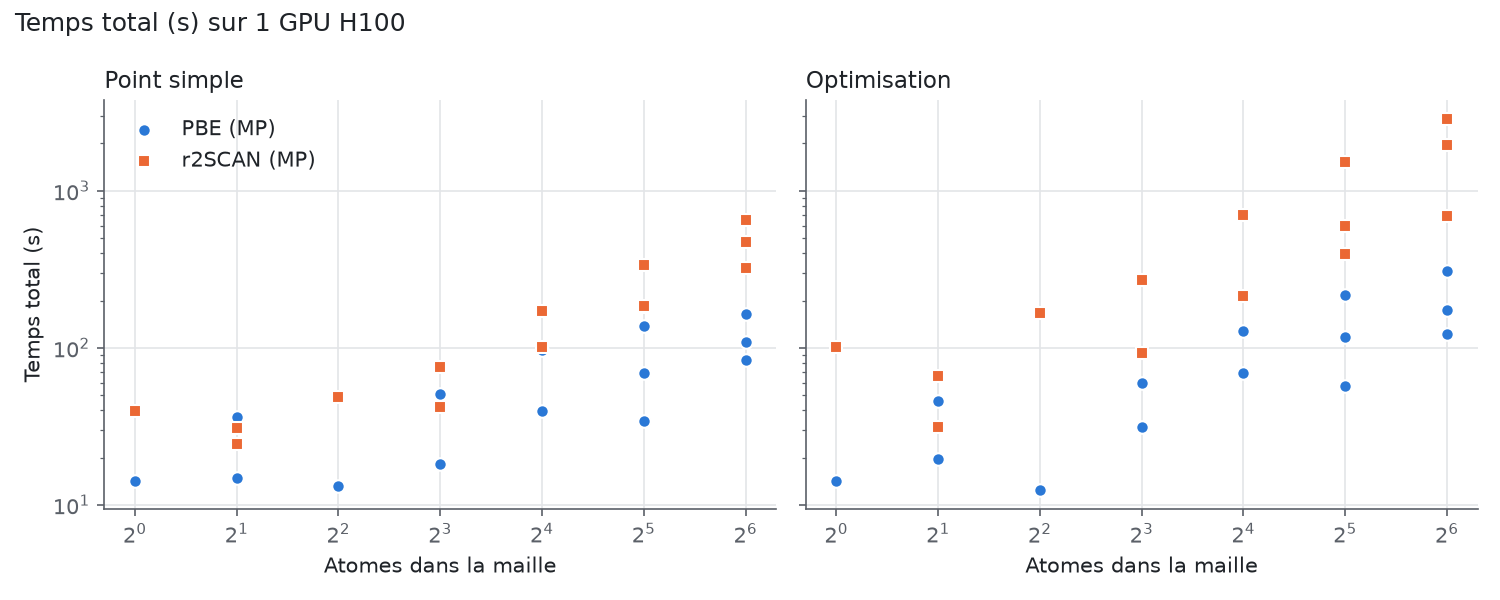
\includegraphics[width=0.8\linewidth]{t_total_vs_natoms.png}
%   \caption{Total time versus number of atoms on one GPU.}
%   \label{fig:t-total}
% \end{figure}

\subsection{Cost of r\textsuperscript{2}SCAN relative to PBE}
\label{sec:res-r2scan}
\todo{Ratios per SCF step and in total, single points and relaxations.}

\subsection{Relaxation versus single point}
\label{sec:res-relax}
\todo{}

\subsection{GPU memory}
\label{sec:res-memory}
\todo{}

\subsection{Reproducibility}
\label{sec:res-repro}
\todo{Relative spread of the three repeats.}

\subsection{Two GPUs: speedup and \texttt{KPAR}}
\label{sec:res-2gpu}
\todo{Final table and Fig.~speedup\_2gpu once phase 4 is complete.}

\subsection{Agreement with Materials Project energies}
\label{sec:res-energies}
\todo{Energy differences per series; explain the PBE offsets for MgO and Al.}

\subsection{Phonons}
\label{sec:res-phonons}
\todo{Dispersions, convergence between supercell sizes, time-to-solution on one and two GPUs.}

% ---------------------------------------------------------------------------
\section{Discussion and Recommendations}
\label{sec:discussion}
\todo{Practical guidance for users of the node: when to request two GPUs, choice of KPAR,
memory headroom, expected run times.}

\section{Conclusion}
\label{sec:conclusion}
\todo{}

\section*{Data and Code Availability}
Scripts, inputs generation, and result tables are available at
\url{https://github.com/John-Akapulco/GPU_vmp_testing_VASP_etc}. VASP output files are kept on
the test machine; PAW potentials are not redistributed, in accordance with the VASP license.

\bibliographystyle{unsrtnat}
\bibliography{references}

\end{document}
